\documentclass[tikz,border=2pt]{standalone}
\usetikzlibrary{arrows.meta,positioning,fit,backgrounds}
\begin{document}
\sffamily\footnotesize
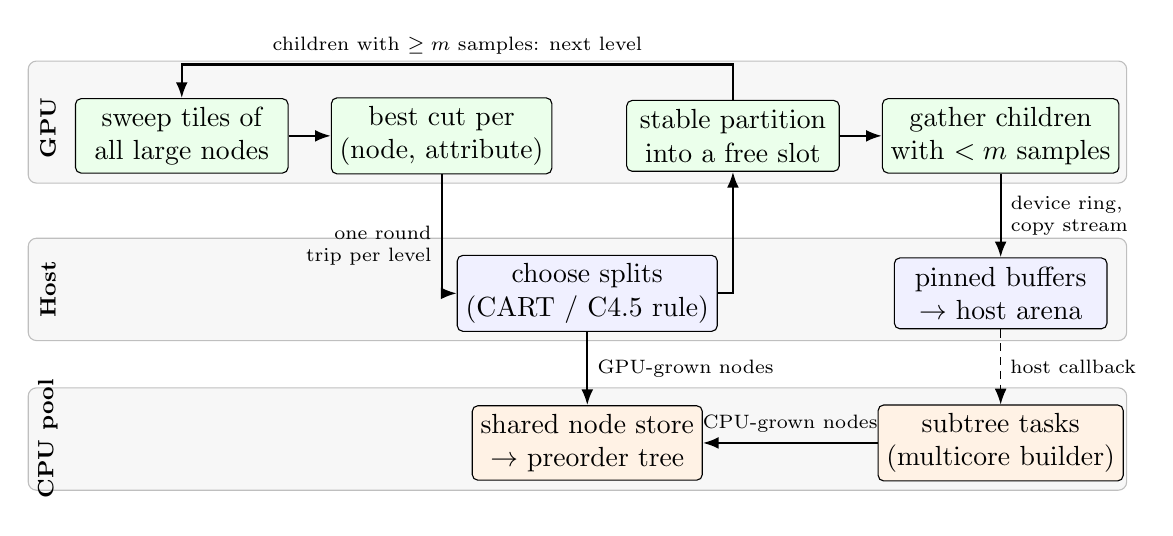
\begin{tikzpicture}[
  box/.style={draw, rounded corners=2pt, align=center, minimum height=9mm,
              minimum width=27mm, inner sep=3pt},
  gpu/.style={box, fill=green!8},
  host/.style={box, fill=blue!6},
  cpu/.style={box, fill=orange!10},
  flow/.style={-{Latex[length=2mm]}, thick},
  ctrl/.style={-{Latex[length=2mm]}, densely dashed},
  lane/.style={draw=black!25, fill=black!3, rounded corners=3pt},
  lbl/.style={rotate=90, font=\bfseries\footnotesize},
  note/.style={font=\scriptsize}]

% node positions (x in cm): three lanes, GPU on top
\node[gpu]  (sweep)  at (0.0, 0)    {sweep tiles of\\all large nodes};
\node[gpu]  (best)   at (3.3, 0)    {best cut per\\(node, attribute)};
\node[gpu]  (part)   at (7.0, 0)    {stable partition\\into a free slot};
\node[gpu]  (gather) at (10.4, 0)   {gather children\\with $<m$ samples};
\node[host] (choose) at (5.15,-2.0) {choose splits\\(CART / C4.5 rule)};
\node[host] (pinned) at (10.4,-2.0) {pinned buffers\\$\rightarrow$ host arena};
\node[cpu]  (store)  at (5.15,-3.9) {shared node store\\$\rightarrow$ preorder tree};
\node[cpu]  (tasks)  at (10.4,-3.9) {subtree tasks\\(multicore builder)};

% lanes
\begin{scope}[on background layer]
  \node[lane, fit={(-1.95,0.95) (12.0,-0.6)}, inner sep=0] (Lg) {};
  \node[lane, fit={(-1.95,-1.3) (12.0,-2.6)}, inner sep=0] (Lh) {};
  \node[lane, fit={(-1.95,-3.2) (12.0,-4.5)}, inner sep=0] (Lc) {};
\end{scope}
\node[lbl] at (-1.7, 0.1)  {GPU};
\node[lbl] at (-1.7,-1.95) {Host};
\node[lbl] at (-1.7,-3.85) {CPU pool};

% GPU level loop
\draw[flow] (sweep) -- (best);
\draw[flow] (best.south) |- node[pos=0.3, left, note, align=right]
  {one round\\trip per level} (choose.west);
\draw[flow] (choose.east) -| (part.south);
\draw[flow] (part) -- (gather);
\draw[flow] (part.north) -- ++(0,0.45) -| node[pos=0.25, above, note]
  {children with $\geq m$ samples: next level} (sweep.north);

% hand-off to the CPU
\draw[flow] (gather) -- node[right, note, align=left] {device ring,\\copy stream} (pinned);
\draw[ctrl] (pinned) -- node[right, note] {host callback} (tasks);

% one tree
\draw[flow] (choose) -- node[right, note] {GPU-grown nodes} (store);
\draw[flow] (tasks) -- node[above, note] {CPU-grown nodes} (store);
\end{tikzpicture}
\end{document}
